% \setlength{\belowcaptionskip}{-1.3cm} %调整图片标题与下文距离 
% \setlength{\abovecaptionskip}{-0.2cm} %调整图片标题与图距离
\begin{figure*}
    \centering
    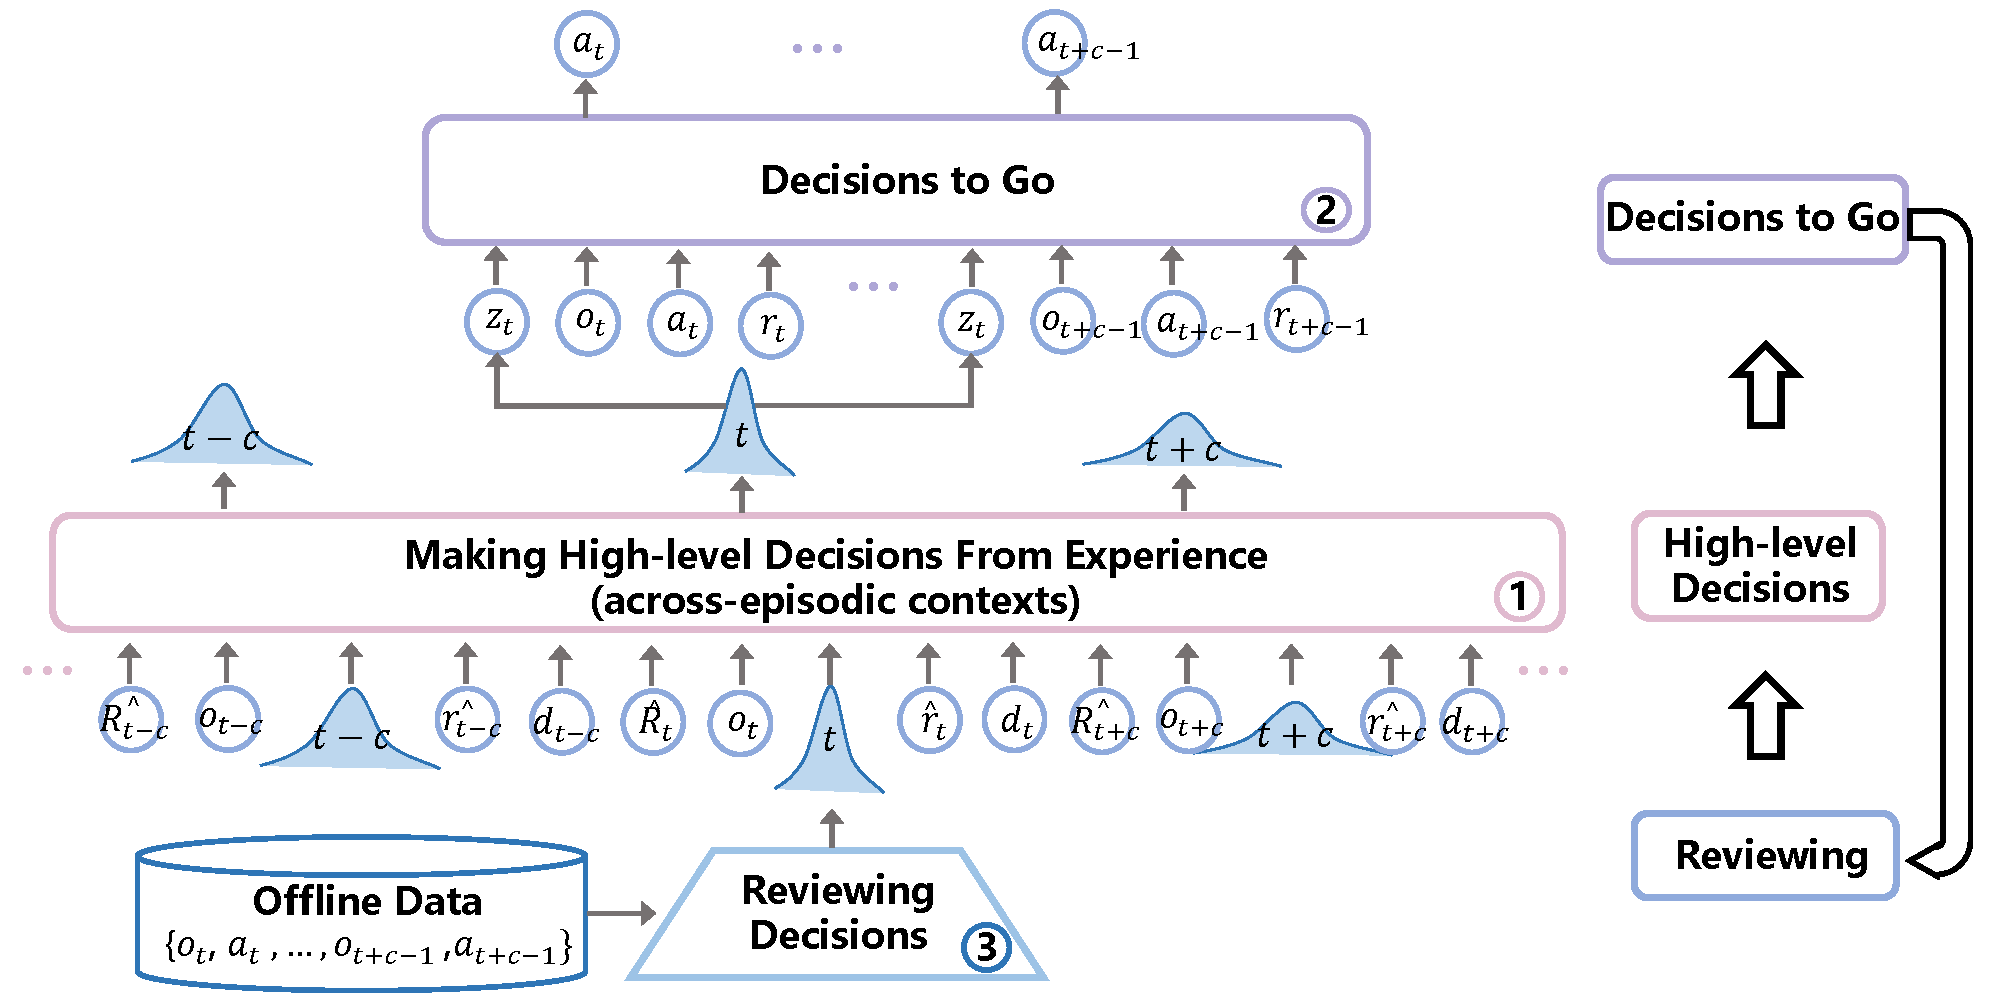
\includegraphics[width=1.7\columnwidth]{results/IDT.pdf}
    \caption{The architecture of IDT is designed into three modules to simulate the high-level trial-and-error process. First, the (1) Making Decisions module predicts a high-level decision by providing across-episodic contexts, where across-episodic contexts contain multiple trajectories arranged in ascending order of the total rewards. Then, the (2) Decisions to Go module predicts actions for $c$ steps conditioned on the predicted high-level decision. Finally, the (3) Reviewing Decisions module reviews the executed actions to serve as an experience for the next cycle. Note that the Reviewing Decisions encodes the true label of high-level decisions from offline data at training while encodes from the executed actions at testing.
    % In particular, the Reviewing Decisions model can not only review its own actions but also the actions from offline data.
    }
    \label{IDT}
\end{figure*}

\section{Method}
In this section, we present IDT, which models a high-level trial-and-error process through a hierarchical chain of experience, as summarized in Figure ~\ref{IDT}.

\subsection{Chain of Experience}
The key factors that influence our modeling on how to represent trajectories are (1) the ability of transformers to uncover meaningful patterns from multiple trajectories and (2) the capacity to improve itself conditioned on experience. The basic elements of trajectories are observations $o$, actions $a$, rewards $r$, and completion token $d$. As modeling rewards is a nontrivial task, we aim to have the model generate actions based on the target returns $\hat{R}_0$ \cite{2}, which can be updated using rewards $\hat{R}_t=\hat{R}_0-\sum_{j=0}^tr_j$. Therefore, the following trajectory representation is amenable to autoregressive training and generation:
\begin{equation}
    \tau = (\hat{R}_0,o_0,a_0,r_0,d_0,\dots,\hat{R}_T,o_T,a_T,r_T,d_T).
\end{equation}

To facilitate the model to achieve target return, we construct across-episodic contexts that consist of multiple trajectories for self-improvement during test time \cite{1}. This idea arises from the approach called chain of hindsight \cite{24}, which trains language models from human feedback by conditioning on positive indicators and negative-rated examples to predict corresponding positive-rated examples. In the RL tasks, the positive indicator is the target return, and previous trajectories serve as negative-rated examples to predict the trajectory with higher returns.

Specifically, the chain of experience is represented by $n$ trajectories: $s=(\tau^{1},\tau^{2},\dots,\tau^{n})$ where
\begin{equation}
    \tau^{i}= (\hat{R}_0^i,o_0^i,a_0^i,r_0^i,d_0^i,\dots,\hat{R}_T^i,o_T^i,a_T^i,r_T^i,d_T^i).
\label{coe}
\end{equation}

The trajectories are ascending sorted according to their total rewards, i.e., $\sum_{t=0}^T{r_t^1}\leq\sum_{t=0}^T{r_t^2}\leq\dots\leq\sum_{t=0}^T{r_t^n}$. For all $n$ trajectories, the initial target return $\hat{R}_0^i$ equals the max total reward, i.e., the last trajectory $\hat{R}_0^n=\sum_{t=0}^T{r_t^n}$.

\subsection{Hierarchical Chain of Experience}
After building across-episodic contexts based on the chain of experience, in-context RL can automatically improve its performance at evaluation time by rolling trajectories in a trial-and-error manner. However, this suffers substantial computational costs when the horizon of tasks increases.

Since total rewards are obtained at the end of episodes, it is more difficult to evaluate and improve a policy model in long-horizon tasks. In traditional RL methods, an effective solution is to decompose complex tasks into several sub-problems by incorporating hierarchical structures  \cite{10}. The high-level policy only needs to generate a signal once to control the low-level policy to generate multi-step actions. This allows (1) the high-level policy to receive feedback faster, as if working on a short-horizon task, and (2) the low-level policy only needs to consider how to better implement the sub-tasks generated by the high-level decision. Although the hierarchical structure can be optimized end-to-end by reward signals, the trial-and-error process in in-context RL is more complicated.

As psychologist Edward Thorndike mentioned, the trial-and-error process includes two parts \cite{16}, memory and search. The high-level decision plays an important role that is closely connected with memory and search. A high-level decision is generated from the search process and directly affects the quality of low-level executed actions. Subsequently, it also serves as the memory for future searches. Therefore, we designed three modules to realize a high-level trial-and-error process: Making Decisions, Decisions to Go, and Reviewing Decisions.

\noindent\textbf{Making Decisions.}~~
The purpose of the Making Decisions module is to generate high-level decisions autoregressively, where the high-level decision is represented by a vector $\textbf{z}$ sampled from a multivariate Gaussian distribution. As the quality of $\textbf{z}$ directly relates to low-level actions $a$, a better high-level decision $\textbf{z}$ is critical for inducing better low-level actions $a$. Therefore, we reconstruct across-episodic contexts represented as a high-level chain of experience $s_h=(\tau_h^{1},\tau_h^{2},\dots,\tau_h^{n})$. Each $\tau_h^{i}$ is denoted as:
\begin{equation}
\begin{aligned}
\tau_h^{i}=(&\hat{R}_0^i,o_0^i,\textbf{z}_0^i,\hat{r}_0^i,d_0^i,\hat{R}_{c}^i,o_{c}^i,\textbf{z}_{c}^i,\hat{r}_{c}^i,d_{c}^i,\\
&\dots,\hat{R}_{kc}^i,o_{kc}^i,\textbf{z}_{kc}^i,\hat{r}_{kc}^i,d_{kc}^i),
\label{hcoe}
\end{aligned}
\end{equation}
where each high-level decision $\textbf{z}$ is generated every $c$ steps, $T-c\leq kc \leq T$, and $\hat{r}_c^i=\sum_{t=c}^{2c-1}{r_t^i}$ is the sum of $c$ steps rewards. By comparing with Equation \eqref{coe}, the high-level chain of experience can considerably shorten the length of contexts and, therefore, significantly alleviate the computational complexity of the self-attention mechanism.

\noindent\textbf{Decisions to Go.}~~
Based on high-level decisions, the Decisions to Go module is designed to generate low-level actions that can interact with environments. Since the transformer-based policy is a conditional generative model, we can build a low-level context that contains high-level decisions to control the low-level actions. The low-level context is represented as:
\begin{equation}
\begin{aligned}
\tau_l^{i,j}=&(\textbf{z}_j^i,o_j^i,a_j^i,r_j^i, \textbf{z}_{j}^i,o_{j+1}^i,a_{j+1}^i,r_{j+1}^i, \\ &\dots,\textbf{z}_{j}^i,o_{j+c-1}^i,a_{j+c-1}^i,r_{j+c-1}^i),
\label{lcoe}
\end{aligned}
\end{equation}
where each $\tau_l^{i,j}$ starts from the generation step $j\in\{0,c,\dots,kc\}$ of high-level decisions and completes $c$ steps low-level actions in the trajectory $\tau^i$. In particular, we introduce the reparameterization trick \cite{20} into high-level decisions to ensure backpropagation through the Decisions to Go module to the Making Decisions module. 

\noindent\textbf{Reviewing Decisions.}~~
% Since the trial-and-error process relies on a conditional generated model, action labels for each step in the trajectory are necessary during training.
The autoregressive training of the conditional generation model is achieved by predicting each token in the sequence. 
For example, when the transformer model is trained to generate $a_t$, we need to provide the action label at time $t$ and condition it on the historical actions $\{a_0,\dots,a_{t-1}\}$. However, the supervisory signals about high-level decisions $\textbf{z}$ are not directly observable from the sequence, as shown in Equation~\eqref{hcoe}. For instance, when the transformer model is trained to generate $\textbf{z}_{j}$ ($j\in\{0,c,\dots,kc\}$), we have neither the true label of $\textbf{z}_{j}$ nor the previous high-level decisions $\{\textbf{z}_0,\textbf{z}_c,\dots,\textbf{z}_{j-c}\}$. 

To this end, we replace the true label of $\textbf{z}_{j}$ with the gradients from the Decisions to Go module trained to generate the following $c$ steps of actions $\{a_{j},a_{j+1},\dots,a_{j+c-1}\}$. For the previous high-level decisions $\{\textbf{z}_0,\textbf{z}_c,\dots,\textbf{z}_{j-c}\}$, we introduce the Reviewing Decisions module to encode the label from low-level actions. 
As the high-level decisions induce low-level actions, the low-level actions should be able to infer high-level decisions inversely. Specifically, to infer a previous high-level decision $\textbf{z}_t \in \{\textbf{z}_0,\textbf{z}_c,\dots,\textbf{z}_{j-c}\}$, we first utilize the self-attention operation to aggregate the information of $a_{t+c-1}$ and $\{o_t,a_t,\dots,o_{t+c-1},a_{t+c-1}\}$. Then, we apply a linear layer to encode $\textbf{z}_t$ from the aggregated information. Note that the Reviewing Decision module is not required to perform autoregressive generation, so any sequence model, such as LSTM, can replace it.

By combining the above three modules, IDT can automatically improve its performance at evaluation time by rolling trajectories in a high-level trial-and-error manner. We now introduce the implementation details of IDT, including architecture, training, and testing.

\begin{figure*}
    \centering
    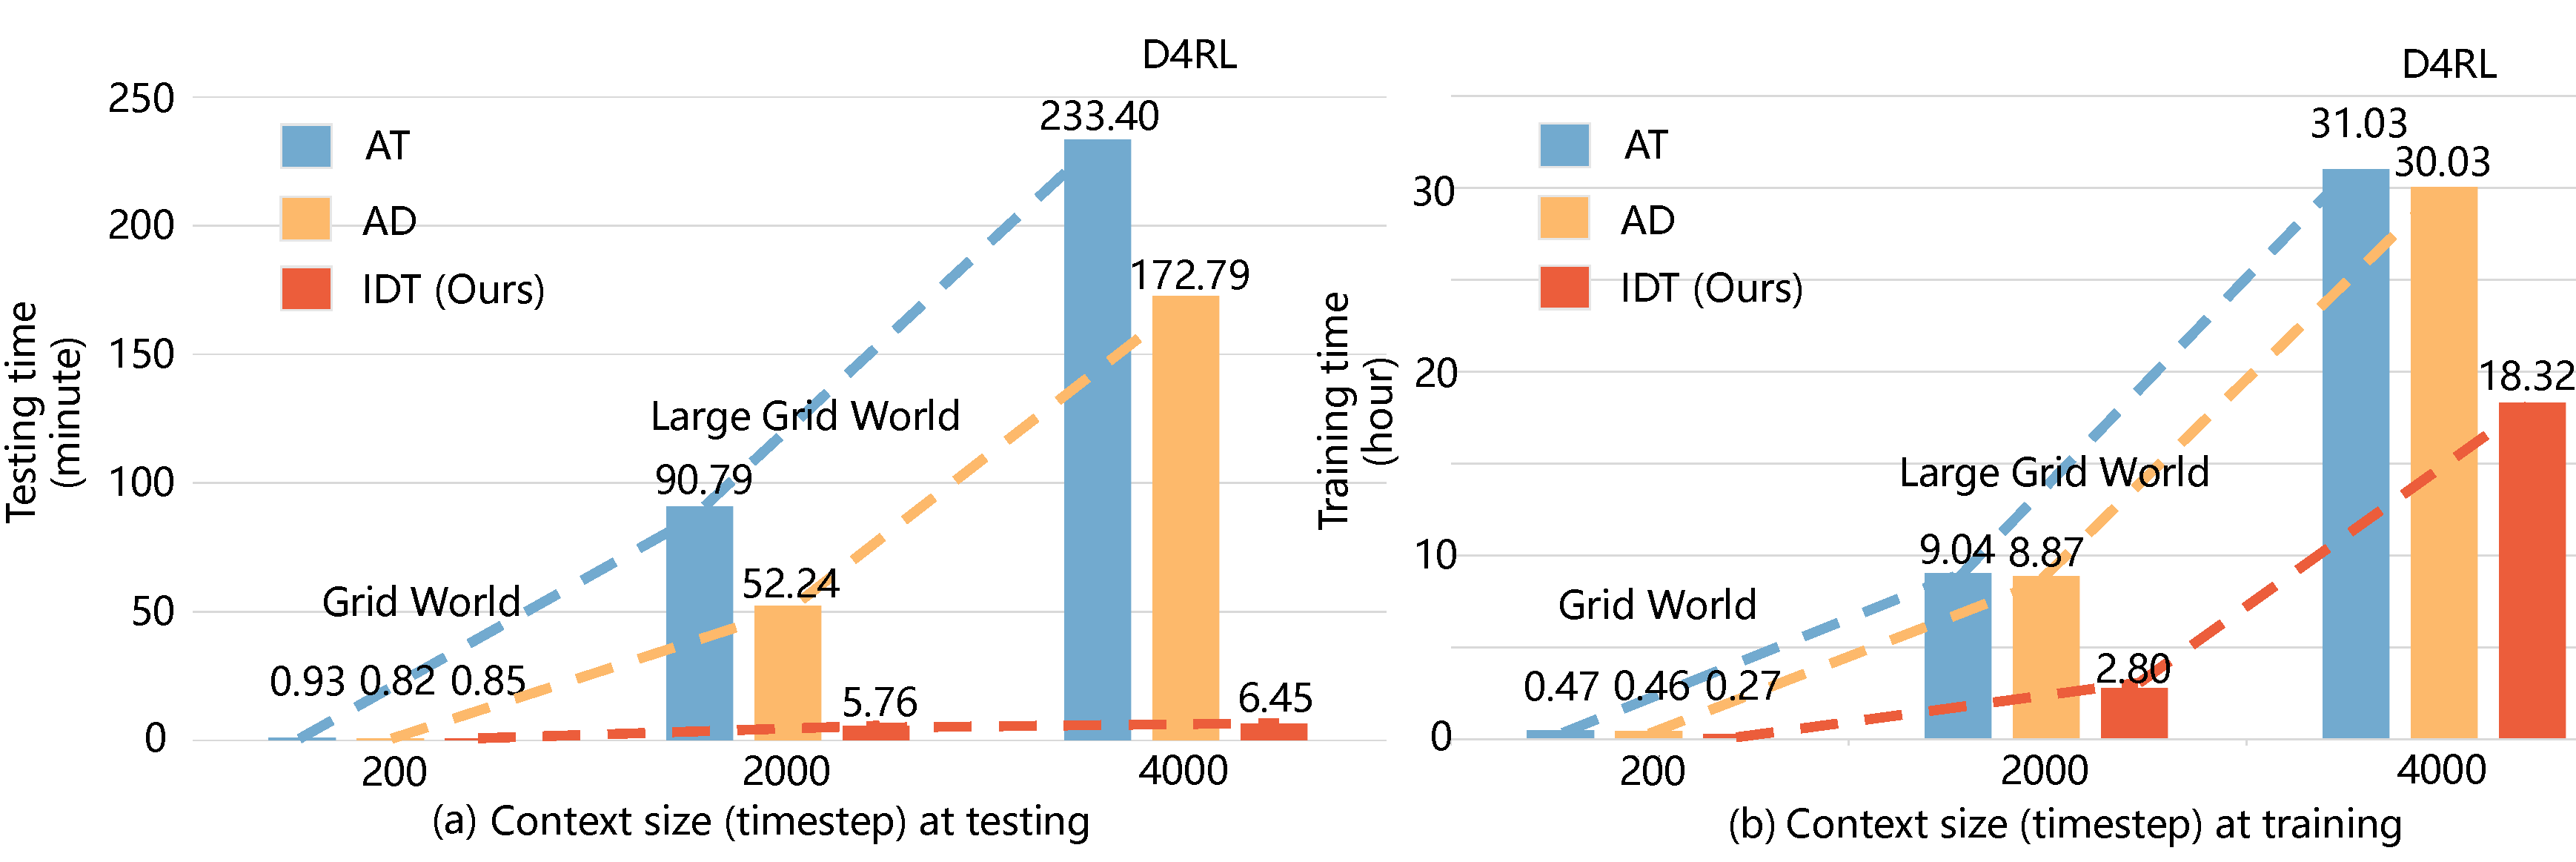
\includegraphics[width=1.9\columnwidth]{results/cost.pdf}
    \caption{Results for (a) testing and (b) training times. We report the training time per 10k gradient updates, the testing time for 50 episodes over Grid World, and 10 episodes over D4RL. Note that we use the number of steps to measure the context size here. The number of tokens per step may vary depending on the algorithm. Each step in AD contains 4 tokens: observation, action, reward, and completion. IDT's Making Decisions module and AT have an extra return-to-go token. As the task length increases, the context length is forced to grow exponentially, resulting in a square increase in computational costs. In contrast, IDT reconstructs the sequence to consist of high-level decisions. Therefore, the context is smaller than one episode length, significantly reducing computational costs.}
    \label{cost_figure}
\end{figure*}



\subsection{Implementation of IDT}

\noindent\textbf{Architecture.}~~
We feed $n$ trajectories into the Making Decisions module, which results in $5\times n\times T/c$ tokens, with one token for each of the five modalities: desired target return, observation, high-level decision, reward, and completion. In the Decisions to Go module, we feed $4\times c$ tokens, with one token for each of the four modalities: high-level decision, observation, action, and rewards. In the Reviewing Decisions module, we feed $2\times c$ tokens, with one token for each of the two modalities: observation and action. To create the token embeddings, we train a linear layer for each modality, which transforms the raw inputs into the desired embedding dimension, followed by layer normalization \cite{26}. Finally, the tokens are processed by a GPT model that predicts future high- and low-level action tokens through autoregressive modeling.

\noindent\textbf{Training and Testing.}~~
During training, we are given a dataset of offline trajectories, where the trajectories can be suboptimal.
In each iteration, we sample minibatches of trajectories from the dataset. 
The Reviewing Decisions module first encodes each true high-level decision $\textbf{z}$ from the minibatch every $c$ steps.
Then, the Making Decisions module predicts the high-level decision $\textbf{z}_t$ given the input token $o_t$ and past trajectories. Finally, the Decisions to Go module autoregressively predicts $c$ steps of low-level actions $\{a_t,\dots,a_{t+c-1}\}$ given $\textbf{z}_t$ and $\{o_t,\dots,o_{t+c-1}\}$. The low-level actions are evaluated with either cross-entropy loss or mean-squared error, depending on whether the actions are discrete or continuous. The losses from each timestep are averaged and updated in all three modules end-to-end. At test time, we roll out the IDT with multiple trajectories and report the largest return among trajectories. Following the configuration from related works \citet{1,8}, we set a context size across $n=4$ episodes.
Note that the task horizons $T$ used in this work range from 20 steps to 1000 steps, and the maximum context size reaches 20000 tokens.
The pseudocode for IDT is summarized in Appendix~\ref{appendix A}. Source code and more hyperparameters are described in Appendix~\ref{appendix B}.